\section{Задание №1 (Вариант 51)}

\subsection{Условие} 

Найти решение задачи линейного программирования геометрически.

\[
    F(x_1, x_2) = 3x_1 + x_2 \to \max(\min)\\
\]

\[
    {\huge{\text{а).}\ }}
    \begin{cases}
        2x_1 + x_2 \leq 2\\
        -x_1 + 3x_2 \leq 3\\
        x_1 \geq 0\\
        x_2 \geq 0
    \end{cases}
    \hspace{1.5cm}
    {\huge{\text{б).}\ }}
    \begin{cases}
        x_1 - 3x_2 \leq 2 \\
        x_1 + x_2 \geq 10 \\
        x_1 \geq 0 \\
        x_2 \geq 0
    \end{cases}
    \hspace{1.5cm}
    {\huge{\text{в).}\ }}
    \begin{cases}
        -x_1 + x_2 \geq 11\\
        x_1 - 4x_2 \geq 8\\
        x_1 \geq 0\\
        x_2 \geq 0
    \end{cases}
\]

\subsection{Решение}

Для всех пунктов нам понадобится знать вектор градиента функции $F(x_1, x_2)$.

\[\overrightarrow{grad}F(x_1, x_2) = \left\{\deriv{F}{x_1}(x_1, x_2), \deriv{F}{x_2}(x_1, x_2)\right\} = \left\{3, 1\right\}\]

\subsubsection{Пункт А}

Приведем неравенство к более наглядному виду, чтобы удобнее было строить график:

\[
    \begin{cases}
        x_2 \leq -2x_1 + 2\\
        x_2 \leq \dfrac{1}{3}x_1 + 1\\
        x_1 \geq 0\\
        x_2 \geq 0
    \end{cases}
\]

Построим график с помощью библиотеки $matplotlib$ для $Python$:\\ \\

\begin{lstlisting}[language=Python, label=code: 01-lab-01-code]
    
    import numpy as np
    import matplotlib.pyplot as plt
    import matplotlib as mpl
    
    plt.rc("text", usetex=True)
    plt.rc(
        "text.latex",
        preamble=r"""
    \usepackage[english, russian]{babel}
    \usepackage[utf8]{inputenc}
    """,
    )
    plt.style.use("seaborn-v0_8")
    
    
    def find_intersection(a1, b1, a2, b2):
        x_1 = (b2 - b1) / (a1 - a2)
        x_2 = a1 * x_1 + b1 if a1 != float("inf") else a2 * x_1 + b2
        return x_1, x_2
    
    
    a1, b1 = -2, 2
    a2, b2 = 1 / 3, 1
    a3, b3 = float("inf"), 0
    a4, b4 = 0, 0
    g1, g2 = 3, 1
    a = [a1, a2, a3, a4]
    b = [b1, b2, b3, b4]
    
    
    X = np.linspace(-20, 100, 1000)
    line1 = a1 * X + b1
    line2 = a2 * X + b2
    line3 = a3 * X + b3
    line3 = np.zeros(1000)
    line4 = a4 * X + b4
    
    fix, ax = plt.subplots()
    plt.quiver(
        0,
        0,
        g1,
        g2,
        angles="xy",
        scale_units="xy",
        scale=1,
        color="black",
        label=r"$\overrightarrow{grad}\ F(x_1,x_2)$",
    )
    
    
    ax.plot(X, line1, label=r"$x_2 = -2x_1 + 2$")
    ax.plot(X, line2, label=r"$x_2 = \frac{1}{3}x_1 + 1$")
    ax.plot(line3, X, label=r"$x_1 = 0$")
    ax.plot(X, line4, label=r"$x_2 = 0$")
    ax.fill_between(
        X, line1, -1, color="blue", alpha=0.2, label="Область $x_2 \leq -2x_1 + 2$"
    )
    ax.fill_between(
        X,
        line2,
        -3,
        color="red",
        alpha=0.2,
        label=r"Область $x_2 \leq \frac{1}{3}x_1 + 1$",
    )
    
    intersections = []
    for i in range(len(a)):
        for j in range(len(a)):
            if i < j:
                intersections += [find_intersection(a[i], b[i], a[j], b[j])]
    
    intersections = [(x_1, x_2) for (x_1, x_2) in intersections if x_1 >= 0 and x_2 >= 0]
    
    for i, (x_1, x_2) in enumerate(intersections, start=1):
        plt.plot(x_1, x_2, 'ko')
        plt.annotate(f'{i}: ({x_1:.2f}, {x_2:.2f})', xy=(x_1, x_2), xytext=(x_1 + 0.3, x_2 + 0.4),
                     arrowprops=dict(facecolor='black', arrowstyle='->'))
    
    ax.set_xlim(-0.01, 3.5)
    ax.set_ylim(-0.01, 3.5)
    ax.set_xlabel(r"$\mathbf{x_1}$", fontsize=12)
    ax.set_ylabel(r"$\mathbf{x_2}$", fontsize=12)
    ax.legend(loc="upper right", fontsize=12, ncol=2)
    plt.gca().set_aspect("equal")
    plt.show()

\end{lstlisting}

Код выше выдаст следующий результат:
\begin{figure}[H]
    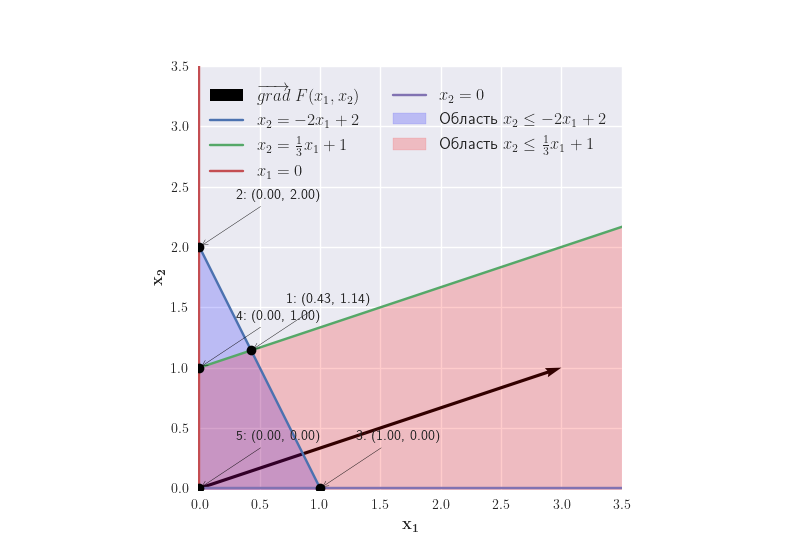
\includegraphics[width=1.0\textwidth]{images/01-lab/01-graphic.png}
    \caption{График к пункту А задания 1.}
    \label{fig:01-lab-01-graphic}
\end{figure}

В условную область попадают все точки, кроме второй. Подставим подходящие точки в функцию $F$ и выведем ее $\max$ и $min$.

\begin{lstlisting}[language=Python]
    def F(x_1, x_2):
        return g1 * x_1 + g2 * x_2

    for i, (x_1, x_2) in enumerate(intersections, start=1):
        if i != 2:
            print(f"Значение F в точке {i} равно {F(x_1, x_2):.2f}")
\end{lstlisting}

Вывод:
\begin{verbatim}
    Значение F в точке 1 равно 2.43
    Значение F в точке 3 равно 3.00
    Значение F в точке 4 равно 1.00
    Значение F в точке 5 равно 0.00
\end{verbatim}

\textbf{Ответ:} $\max F(x_1, x_2) = 3, \argmax F(x_1, x_2) = (1, 1);\\
\min F(x_1, x_2) = 0, \argmin F(x_1, x_2) = (1, 0)$

\subsubsection{Пункт Б}

Приведем неравенство к наглядному виду:

\[
    \begin{cases}
        x_2 \geq \dfrac{1}{3} x_1 - \dfrac{2}{3}\\
        x_2 \geq -x_1 + 10\\
        x_1 \geq 0\\
        x_2 \geq 0
    \end{cases}
\]

Построим график с помощью библиотеки $matplotlib$ для $Python$ (используется код со страницы \pageref{code: 01-lab-01-code}), коэффициенты прямых указаны новые:

\begin{lstlisting}[language=Python]
    a1, b1 = 1 / 3, -2 / 3
    a2, b2 = -1, 10
    a3, b3 = float("inf"), 0
    a4, b4 = 0, 0
    g1, g2 = 3, 1
\end{lstlisting}
Вывод:
\begin{figure}[H]
    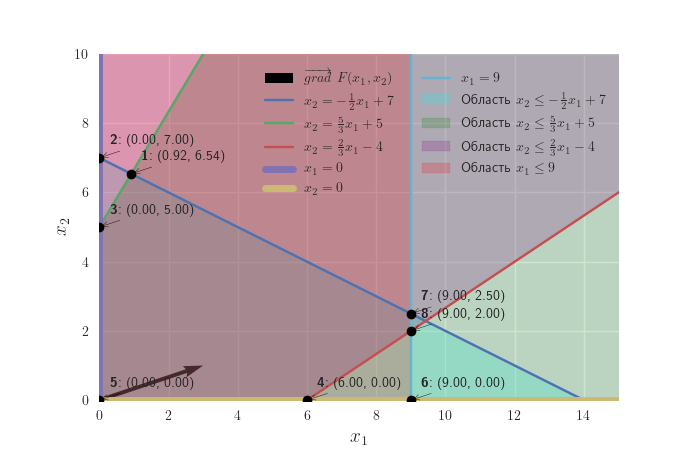
\includegraphics[width=1\textwidth, center]{images/01-lab/02-graphic.png}
    \caption{График к пункту Б задания 1.}
    \label{fig:01-lab-02-graphic}
\end{figure}

Условная область неограничена. Градиент функции направлен внутрь первой четверти. Функция $F$ неограничена сверху. Ее максимума не существует.

Осталось найти минимум $F$. Подходящие точки под номерами 1 и 3. Подставим подходящие точки в функцию $F$ и выведем ее $min$.
\begin{lstlisting}[language=Python]
    def F(x_1, x_2):
        return g1 * x_1 + g2 * x_2


    for i, (x_1, x_2) in enumerate(intersections, start=1):
        if i == 1 or i == 3:
            print(f"Значение F в точке {i} равно {F(x_1, x_2):.2f}")
\end{lstlisting} 
Вывод:
\begin{verbatim}
    Значение F в точке 1 равно 26.00
    Значение F в точке 3 равно 10.00
\end{verbatim}

\textbf{Ответ:} $\max F(x_1, x_2) \notin \R, \argmax F(x_1, x_2) \notin \R^2, \min F(x_1, x_2) = 10, \argmin F(x_1, x_2) = (0, 10)$

\subsubsection{Пункт В}

Приведем неравенство к более наглядному виду:
\[
    \begin{cases}
        x_2 \geq x_1 + 11\\
        x_2 \leq \dfrac{1}{4}x_1 - 2\\
        x_1 \geq 0\\
        x_2 \geq 0
    \end{cases}
\]

Построим график с помощью библиотеки $matplotlib$ для $Python$ (используется код со страницы \pageref{code: 01-lab-01-code}), коэффициенты прямых указаны новые:
\begin{lstlisting}[language=Python]
    a1, b1 = 1, 11
    a2, b2 = 1/4, -2
    a3, b3 = float("inf"), 0
    a4, b4 = 0, 0
    g1, g2 = 3, 1
\end{lstlisting}
Вывод:
\begin{figure}[H]
    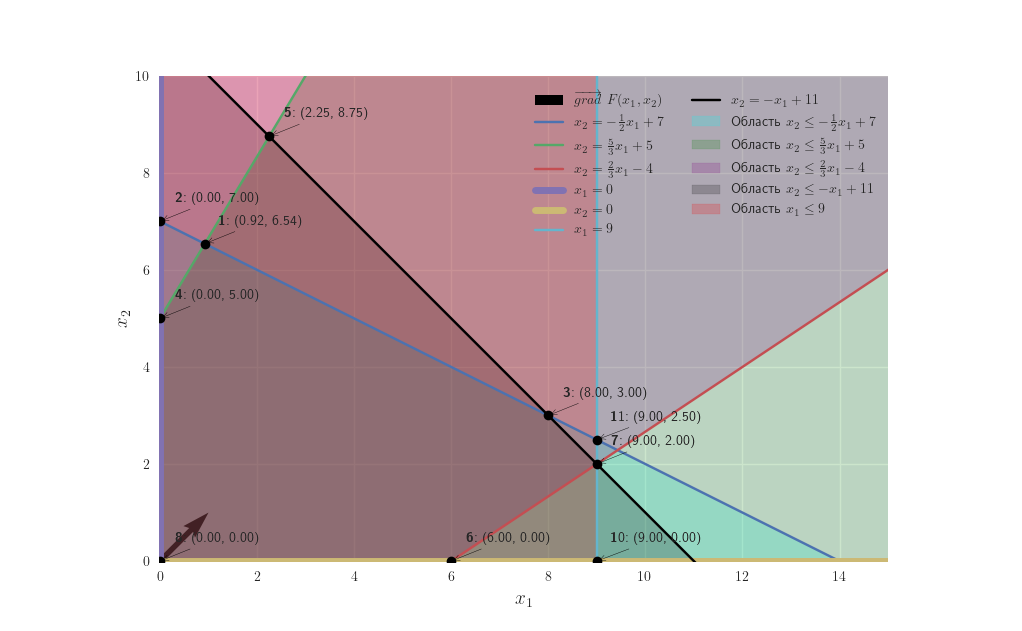
\includegraphics[width=1\textwidth, center]{images/01-lab/03-graphic.png}
    \caption{График к пункту В задания 1.}
    \label{fig:01-lab-03-graphic}
\end{figure}

Как видно, мы имеем пустую условную область: $D = \varnothing$. Значит и $F(D) = \varnothing$. Максимума и минимума не существует.

\textbf{Ответ:} $\nexists\max F(x_1, x_2), \nexists\argmax F(x_1, x_2), \nexists\min F(x_1, x_2), \nexists\argmin F(x_1, x_2)$

\newpage

